As a classical model for paramagnetism one 
can consider a system of $N$ particles with 
the Hamiltonian
\begin{equation}
    \mathcal{H}=-hM
    \ \ \ \textnormal{with}\ \ \ 
    M=\mu\cdot\sum_{i=1}^N\cos\theta_i
\end{equation}
where $h$ is an external homogeneous magnetic 
field, $\mu$ the magnetic moment of a single 
particle and $\theta_i$ the angle between the
magnetic field $h$ and the magnetic moment
$\mu$ of particle $i$.

\paragraph{1. Use the canonical distribution 
    to calculate the average magnetization, 
    $\langle M\rangle$, as a function of $h$
    and temperature $T$. 
    \textit{(3 points)}
} \ \\
    \\
    Partition function:
    \begin{align}
        Z
        &=\frac{1}{h^{3N}}\cdot
        \int d^{3N}r 
        \int d^{3N}p
        \int d^N\Omega\
        e^{-\beta\mathcal{H}} \\
        &=Z_0\cdot\bigg(
            \int_0^{2\pi}d\varphi 
            \int_0^\pi d\theta
            \cdot\sin\theta\cdot 
            e^{h\beta\mu\sum_i^N\cos\theta_i}
        \bigg) \\
        &=Z_0\cdot\bigg(
            \int_0^{2\pi}d\varphi 
            \int_0^\pi d\theta
            \cdot\sin\theta\cdot 
            e^{h\beta\mu\cos\theta}
    \bigg)^N \\
        &=Z_0\cdot\bigg(
            \frac{4\pi\cdot\sinh(\beta\mu h)}
            {\beta\mu h}
        \bigg)^N
    \end{align}
    Free energy:
    \begin{align}
        F
        &=-k_BT\ln(Z) \\
        &=-k_BT\cdot(\ln(Z_0)+N\ln(4\pi))
        -Nk_BT\ln\bigg(
            \frac{\sinh(\beta\mu h)}{\beta\mu h}
        \bigg)
    \end{align}
    Magnetization:
    \begin{align}
        M
        =-\pder{F}{h}\bigg|_{T,V,N}
        =N\mu\cdot\bigg(\coth(x)
        -\frac{1}{x}\bigg)
    \end{align}
    with $x=\beta\mu h$.

\newpage
\paragraph{2. The ratio of which quantities 
    determines the average magnetization? 
    Sketch the functional dependence of the 
    average magnetization on this ratio. 
    \textit{(1 point)}
} \ \\
    \\
    The average magnetization is determined by 
    the ratio $\beta\mu h=\mu h/k_BT$.

    \begin{figure}[h!]
        \centering
        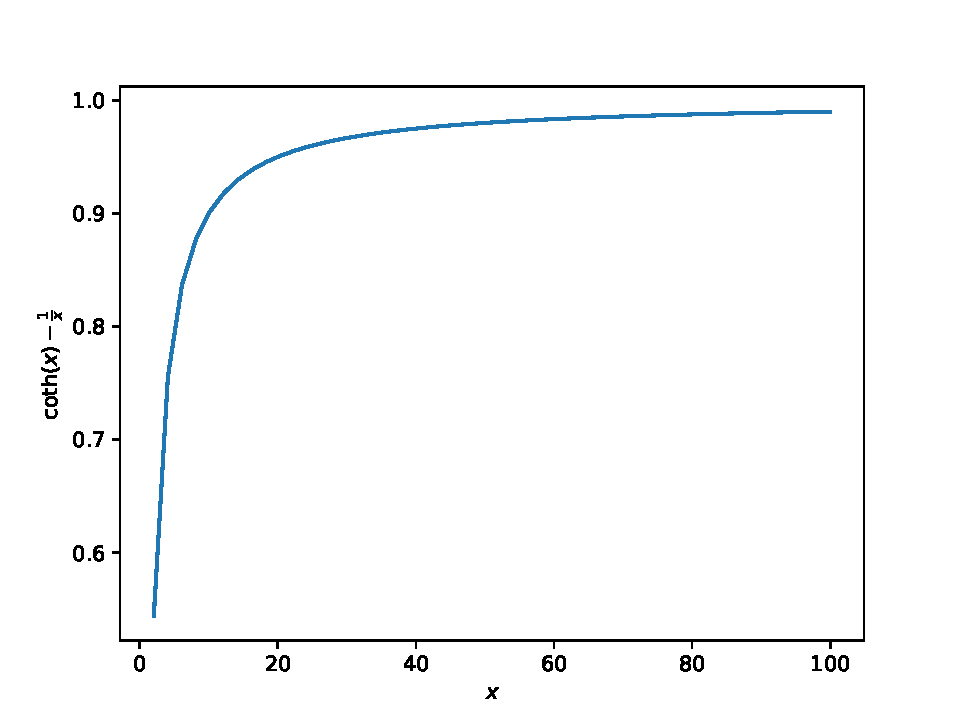
\includegraphics[width=.6\textwidth]{./figures/magnetization.pdf}
    \end{figure} \ \\ 

\paragraph{3. Discuss the two limiting cases: 
    high temperature/weak field vs. 
    low temperature/strong field.
    \textit{(2 points)}
} \ \\
    \\
